\documentclass[ignorenonframetext,]{beamer}
\setbeamertemplate{caption}[numbered]
\setbeamertemplate{caption label separator}{: }
\setbeamercolor{caption name}{fg=normal text.fg}
\beamertemplatenavigationsymbolsempty
\usepackage{lmodern}
\usepackage{amssymb,amsmath}
\usepackage{ifxetex,ifluatex}
\usepackage{fixltx2e} % provides \textsubscript
\ifnum 0\ifxetex 1\fi\ifluatex 1\fi=0 % if pdftex
  \usepackage[T1]{fontenc}
  \usepackage[utf8]{inputenc}
\else % if luatex or xelatex
  \ifxetex
    \usepackage{mathspec}
  \else
    \usepackage{fontspec}
  \fi
  \defaultfontfeatures{Ligatures=TeX,Scale=MatchLowercase}
\fi
% use upquote if available, for straight quotes in verbatim environments
\IfFileExists{upquote.sty}{\usepackage{upquote}}{}
% use microtype if available
\IfFileExists{microtype.sty}{%
\usepackage{microtype}
\UseMicrotypeSet[protrusion]{basicmath} % disable protrusion for tt fonts
}{}
\newif\ifbibliography
\hypersetup{
            pdftitle={Linear Mixed Effects Model},
            pdfborder={0 0 0},
            breaklinks=true}
\urlstyle{same}  % don't use monospace font for urls
\usepackage{color}
\usepackage{fancyvrb}
\newcommand{\VerbBar}{|}
\newcommand{\VERB}{\Verb[commandchars=\\\{\}]}
\DefineVerbatimEnvironment{Highlighting}{Verbatim}{commandchars=\\\{\}}
% Add ',fontsize=\small' for more characters per line
\usepackage{framed}
\definecolor{shadecolor}{RGB}{248,248,248}
\newenvironment{Shaded}{\begin{snugshade}}{\end{snugshade}}
\newcommand{\KeywordTok}[1]{\textcolor[rgb]{0.13,0.29,0.53}{\textbf{#1}}}
\newcommand{\DataTypeTok}[1]{\textcolor[rgb]{0.13,0.29,0.53}{#1}}
\newcommand{\DecValTok}[1]{\textcolor[rgb]{0.00,0.00,0.81}{#1}}
\newcommand{\BaseNTok}[1]{\textcolor[rgb]{0.00,0.00,0.81}{#1}}
\newcommand{\FloatTok}[1]{\textcolor[rgb]{0.00,0.00,0.81}{#1}}
\newcommand{\ConstantTok}[1]{\textcolor[rgb]{0.00,0.00,0.00}{#1}}
\newcommand{\CharTok}[1]{\textcolor[rgb]{0.31,0.60,0.02}{#1}}
\newcommand{\SpecialCharTok}[1]{\textcolor[rgb]{0.00,0.00,0.00}{#1}}
\newcommand{\StringTok}[1]{\textcolor[rgb]{0.31,0.60,0.02}{#1}}
\newcommand{\VerbatimStringTok}[1]{\textcolor[rgb]{0.31,0.60,0.02}{#1}}
\newcommand{\SpecialStringTok}[1]{\textcolor[rgb]{0.31,0.60,0.02}{#1}}
\newcommand{\ImportTok}[1]{#1}
\newcommand{\CommentTok}[1]{\textcolor[rgb]{0.56,0.35,0.01}{\textit{#1}}}
\newcommand{\DocumentationTok}[1]{\textcolor[rgb]{0.56,0.35,0.01}{\textbf{\textit{#1}}}}
\newcommand{\AnnotationTok}[1]{\textcolor[rgb]{0.56,0.35,0.01}{\textbf{\textit{#1}}}}
\newcommand{\CommentVarTok}[1]{\textcolor[rgb]{0.56,0.35,0.01}{\textbf{\textit{#1}}}}
\newcommand{\OtherTok}[1]{\textcolor[rgb]{0.56,0.35,0.01}{#1}}
\newcommand{\FunctionTok}[1]{\textcolor[rgb]{0.00,0.00,0.00}{#1}}
\newcommand{\VariableTok}[1]{\textcolor[rgb]{0.00,0.00,0.00}{#1}}
\newcommand{\ControlFlowTok}[1]{\textcolor[rgb]{0.13,0.29,0.53}{\textbf{#1}}}
\newcommand{\OperatorTok}[1]{\textcolor[rgb]{0.81,0.36,0.00}{\textbf{#1}}}
\newcommand{\BuiltInTok}[1]{#1}
\newcommand{\ExtensionTok}[1]{#1}
\newcommand{\PreprocessorTok}[1]{\textcolor[rgb]{0.56,0.35,0.01}{\textit{#1}}}
\newcommand{\AttributeTok}[1]{\textcolor[rgb]{0.77,0.63,0.00}{#1}}
\newcommand{\RegionMarkerTok}[1]{#1}
\newcommand{\InformationTok}[1]{\textcolor[rgb]{0.56,0.35,0.01}{\textbf{\textit{#1}}}}
\newcommand{\WarningTok}[1]{\textcolor[rgb]{0.56,0.35,0.01}{\textbf{\textit{#1}}}}
\newcommand{\AlertTok}[1]{\textcolor[rgb]{0.94,0.16,0.16}{#1}}
\newcommand{\ErrorTok}[1]{\textcolor[rgb]{0.64,0.00,0.00}{\textbf{#1}}}
\newcommand{\NormalTok}[1]{#1}
\usepackage{graphicx,grffile}
\makeatletter
\def\maxwidth{\ifdim\Gin@nat@width>\linewidth\linewidth\else\Gin@nat@width\fi}
\def\maxheight{\ifdim\Gin@nat@height>\textheight0.8\textheight\else\Gin@nat@height\fi}
\makeatother
% Scale images if necessary, so that they will not overflow the page
% margins by default, and it is still possible to overwrite the defaults
% using explicit options in \includegraphics[width, height, ...]{}
\setkeys{Gin}{width=\maxwidth,height=\maxheight,keepaspectratio}

% Prevent slide breaks in the middle of a paragraph:
\widowpenalties 1 10000
\raggedbottom

\AtBeginPart{
  \let\insertpartnumber\relax
  \let\partname\relax
  \frame{\partpage}
}
\AtBeginSection{
  \ifbibliography
  \else
    \let\insertsectionnumber\relax
    \let\sectionname\relax
    \frame{\sectionpage}
  \fi
}
\AtBeginSubsection{
  \let\insertsubsectionnumber\relax
  \let\subsectionname\relax
  \frame{\subsectionpage}
}

\setlength{\parindent}{0pt}
\setlength{\parskip}{6pt plus 2pt minus 1pt}
\setlength{\emergencystretch}{3em}  % prevent overfull lines
\providecommand{\tightlist}{%
  \setlength{\itemsep}{0pt}\setlength{\parskip}{0pt}}
\setcounter{secnumdepth}{0}
\usepackage{amsmath}
\usetheme{default}
 \definecolor{greenmain}{HTML}{28B478}
 \definecolor{brick}{rgb}{.85,.1,.2}
 \colorlet{greenstruct}{greenmain!87.5!black}
 \usecolortheme[named=greenstruct]{structure}
 % Change this in order to make the presentation look
 % different. Works just like a powerpoint template.
 % Have your RA mess around until it looks nice.
 \setbeamercovered{dynamic}
 \useinnertheme{rectangles}
 \definecolor{bluemain}{HTML}{0B61A4}
 \definecolor{orangemain}{HTML}{FF9200}
 \definecolor{redmain}{HTML}{FF4900}
 \definecolor{redlight}{HTML}{FF9B73}
 \definecolor{orangelight}{HTML}{FFC373}
 \definecolor{cmugray}{RGB}{104,104,104}
 \definecolor{cmulightgray}{RGB}{238,238,238}
 \setbeamercolor{block body}{bg=cmulightgray}
 \setbeamercolor{talktitle}{bg=greenstruct,fg=white}
 \setbeamercolor{block title alerted}{bg=orangemain}
 \setbeamercolor{block body alerted}{bg=orangelight}
%\setbeamertemplate{itemize subitem}{\hbox{\donotcoloroutermaths$\boldsymbol{-}$}}

\setbeamertemplate{blocks}[default]
\setbeamertemplate{navigation symbols}{}
%\usefonttheme{structuresmallcapsserif}

\title{Linear Mixed Effects Model}
\author{Monte Carlo Group\\[2\baselineskip]Liang Zou, Michael Mcbride, Xinlu
Zhang\\
Caleb Donoho, Ashley Lu\\}
\date{22 January 2018}

\begin{document}
\frame{\titlepage}

\begin{frame}{Introduce the definition of LMM}

Linear mixed effects models simply model the fixed and random effects as
having a linear form. Similar to the Generalized Linear Model, an
outcome variable is contributed to by additive fixed and random effects
(as well as an error term). Using the familiar notation, the linear
mixed effect model takes the form:
\[y_{ij}=b_0+b_1x_{ij}+v_i+\epsilon_{ij}\]

\begin{itemize}
\tightlist
\item
  \(y_{ij}\) is the response value for a particular ij case.
\item
  \(b_0\) is fixed intercept for regression model.
\item
  \(b_1\) is fixed slope for regression model.
\item
  \(x_{ij}\) is fixed-effect variable for observation j-th measurement
  of i-th subject.
\item
  \(v_{i}\) is random intercept of i-th subject.
\item
  \(\epsilon_{ij}\) is a Gussian error term which assumed to be
  multivariate normally distributed.
\end{itemize}

\end{frame}

\begin{frame}{Assumption of the models}

\begin{itemize}
\tightlist
\item
  The relationship between x and y is linear
\item
  \(Y\) is observed random variables
\item
  \(X\) is design matrix for fixed effect.
\item
  \(v_i \sim N(0,\sigma^2_v)\) is an unobserved random noise.
\item
  \(\epsilon_i \sim N(0,\sigma^2_\epsilon)\) is an unobserved random
  noise.
\item
  \(v_i\) and \(\epsilon_{ij}\) are independent of each other.
\item
  \(b_0\) and \(b_1\) are unknown constants.
\end{itemize}

\end{frame}

\begin{frame}{When and Why LMM is necessary and carried out.}

We use Linear Mixed Effect Models when we believe that the data comes
from partitions on the sample space, that each partition is internally
correlated, and that the partition means are determined by some global
parameters plus some noise. This type of situation is illustrated on the
graph shown below (image obtained from
\href{https://hlplab.wordpress.com/2011/05/31/mixed-models-and-simpsons-paradox/}{here}):

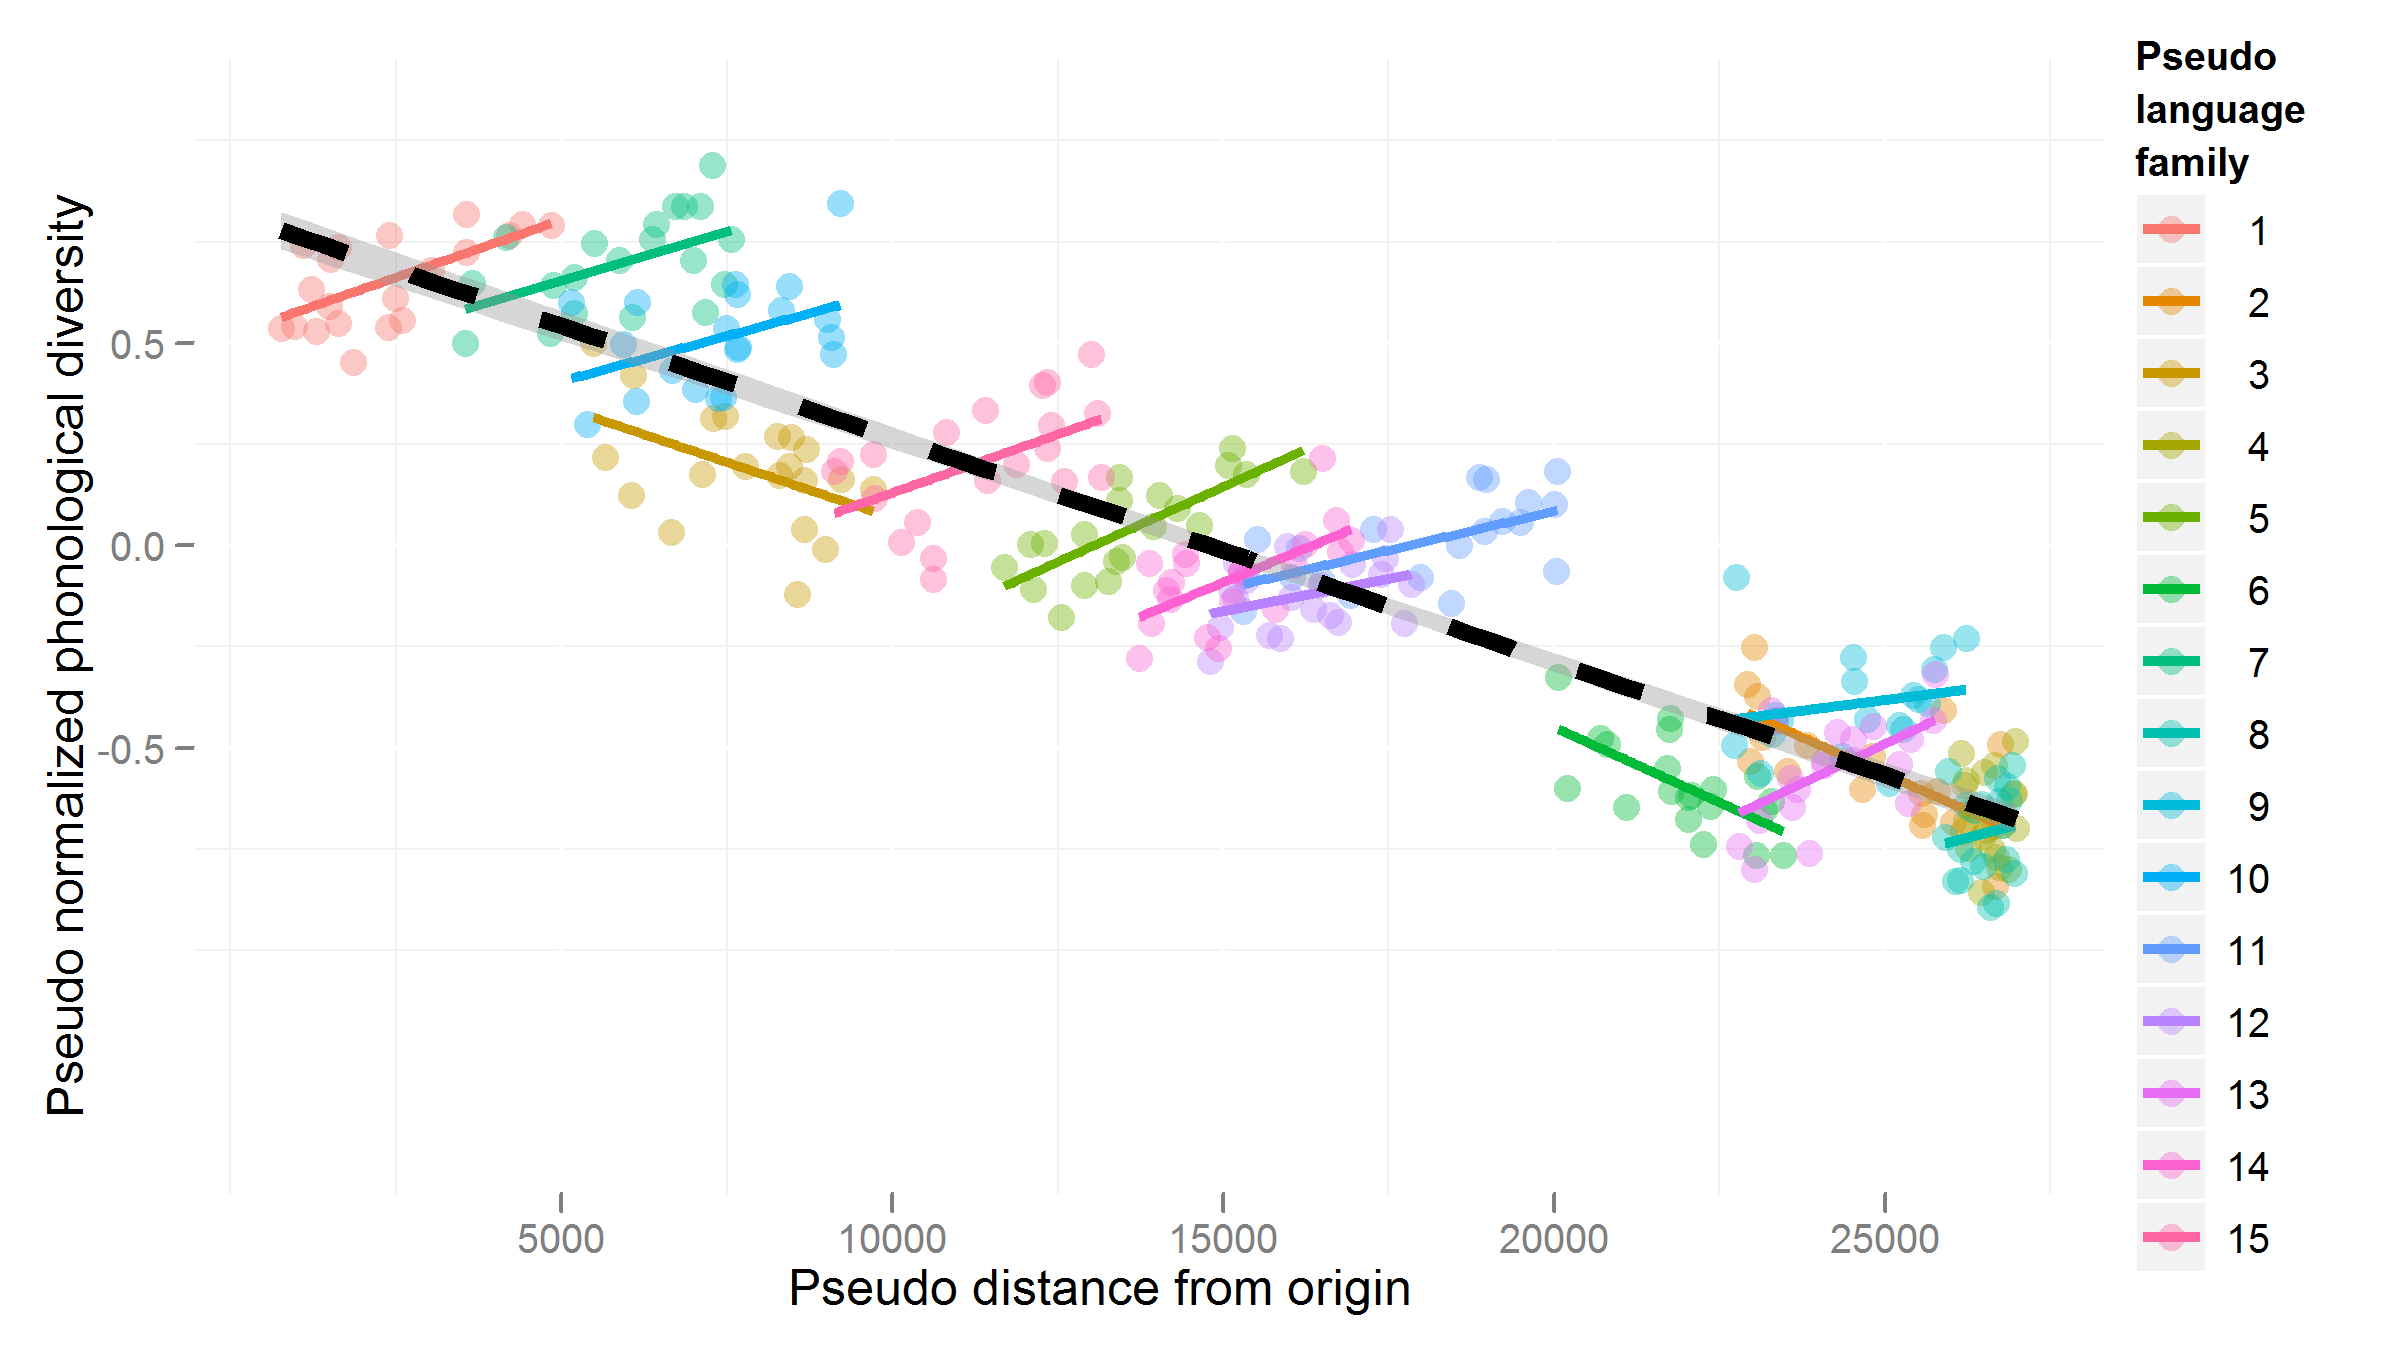
\includegraphics{situation.png}

\end{frame}

\begin{frame}{When and Why LMM is necessary and carried out.}

As we can see, the mean within each group follows the larger line, while
the data within each group follows it's own sub-population line. In
situations like these we might want to be able to make both population
and sub-population inferences, or discuss how much the grouping affects
the variation. Using an LMM allows us do all of these things.
Essentially, we use LMMs when we believe the response variable is
sampled from different distributions, the parameters for which are
sampled from a parent distribution, and we want our inference to be
reflective of this model.

\end{frame}

\begin{frame}[fragile]{Statistical Analysis package and dataset.}

There are several packages in R, which contains for fitting LMMs, for
instance nlme,lme4.0, or MCMCglmm. For use in R, it should be noted that
lme4 and nlme do not interact well with each other.

\begin{Shaded}
\begin{Highlighting}[]
\KeywordTok{require}\NormalTok{(lme4)}
\KeywordTok{citation}\NormalTok{(}\StringTok{"lme4"}\NormalTok{)}
\KeywordTok{require}\NormalTok{(nlme)}
\KeywordTok{citation}\NormalTok{(}\StringTok{"nlme"}\NormalTok{)}
\KeywordTok{require}\NormalTok{(MCMCglmm)}
\KeywordTok{citation}\NormalTok{(}\StringTok{"MCMCglmm"}\NormalTok{)}
\end{Highlighting}
\end{Shaded}

\end{frame}

\begin{frame}{Statistical Analysis package and dataset.}

\end{frame}

\begin{frame}{Perform dataset}

We are using the dataset called lmm.dataRC and using SPSS to perform the
analysis. 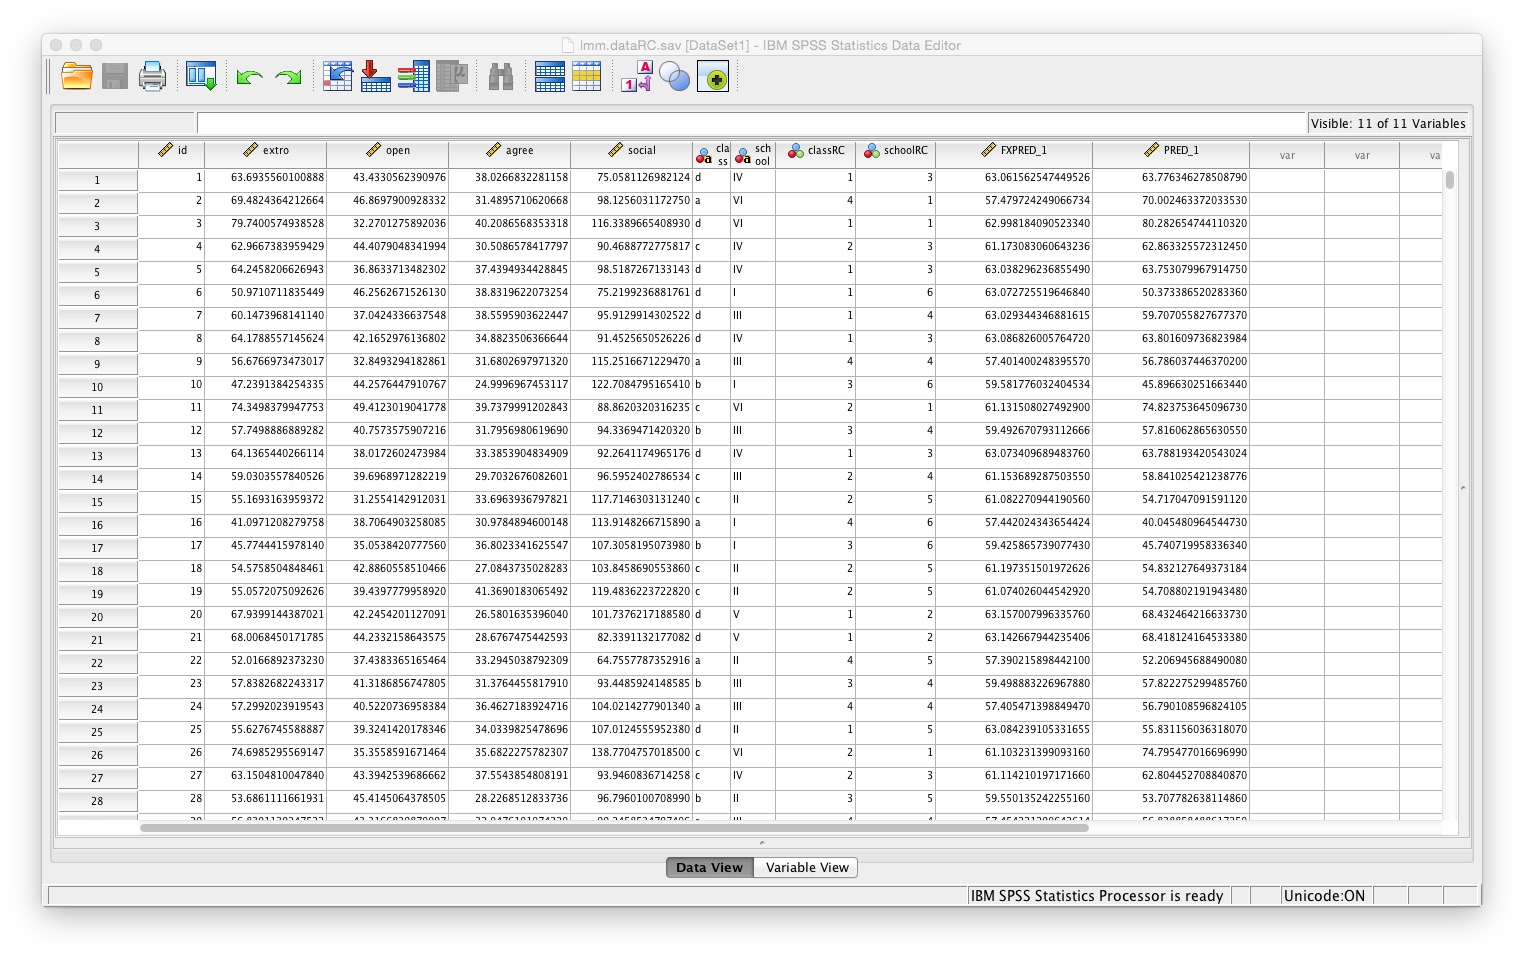
\includegraphics{Dataset1.jpeg}\\

\end{frame}

\begin{frame}{Perform dataset}

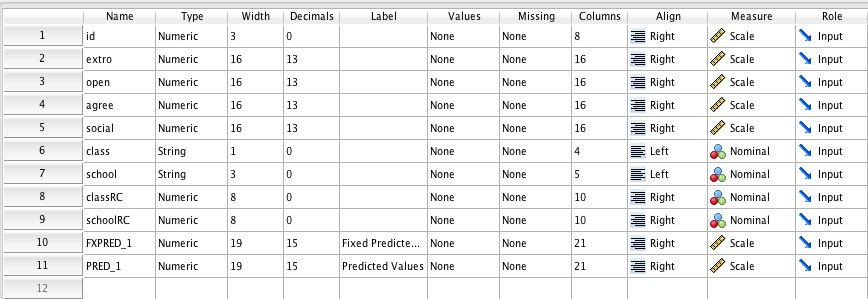
\includegraphics{Dataset2.jpeg}\\

\end{frame}

\begin{frame}{Perform dataset}

\begin{itemize}
\tightlist
\item
  The data contains 1200 cases evenly distributed among 24 nested groups
  (4 classes within 6 schools).
\item
  extro: the interval scaled outcome variable Extroversion.
\item
  open: predicted by fixed effects for the interval scaled predictor
  Openness to new experiences.
\item
  agree: the interval scaled predictor Agreeableness.
\item
  social: the interval scaled predictor Social engagement.
\item
  classRC: the nominal scaled predictor Class.
\item
  schoolRC: the random (nested) effect of Class (classRC) within School
  (schoolRC) as well as the random effect of School.
\end{itemize}

\end{frame}

\begin{frame}{Performance Linear Mixed Effect Model.}

The Case Processing Summary simply shows that the cases are balanced
among the categories of the categorical variables and no cases were
excluded. 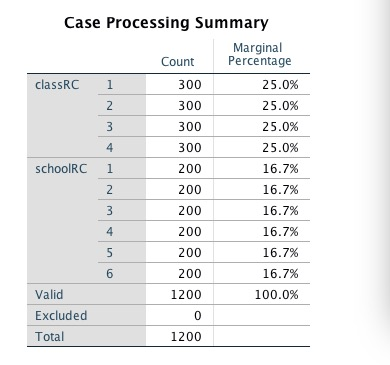
\includegraphics{Case Processing Summary.jpeg}\\

\end{frame}

\begin{frame}{Syntax and interpret of Linear Mixed Effect Model.}

Rather large table contains all the descriptive statistics (only the
very top of the table is shown here).
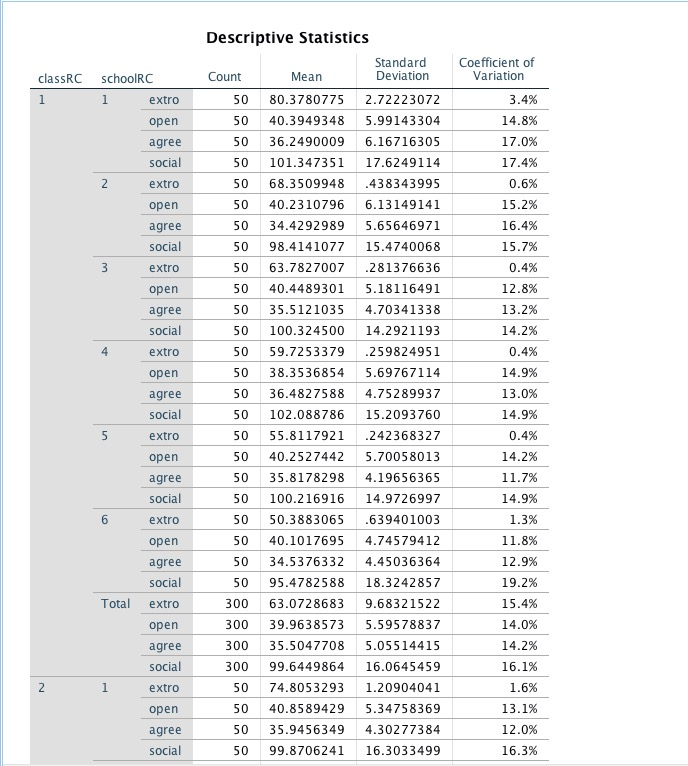
\includegraphics{Descriptive data.jpeg}\\

\end{frame}

\begin{frame}{Syntax and interpret of Linear Mixed Effect Model.}

The Model Dimension table simply shows the model in terms of which
variables (and their number of levels) are fixed and / or random effects
and the number of parameters being estimated
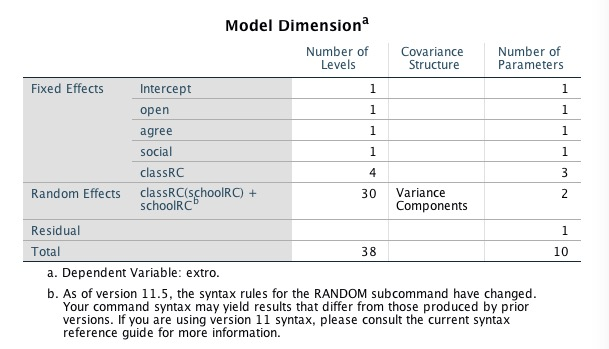
\includegraphics{model dimension.jpeg}\\

\end{frame}

\begin{frame}{Syntax and interpret of Linear Mixed Effect Model.}

The table displays fit indices. For each index; the lower the number,
the better the model fits the data.

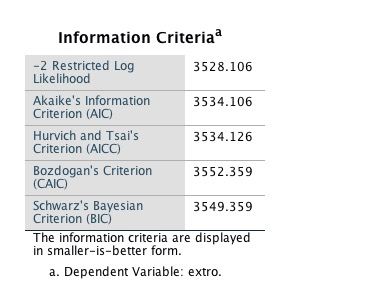
\includegraphics{information criteria.jpeg}\\

\end{frame}

\begin{frame}{Syntax and interpret of Linear Mixed Effect Model.}

This table is our Estimates of Fixed Effect. This is what we'd expect to
see in a normal linear regression model with our \(\beta\) values, their
standard error, degrees of freedom, t-value, significance, and 95\%
interval.\\
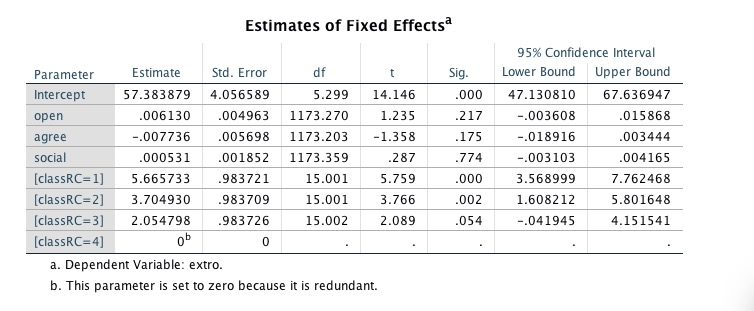
\includegraphics{estimates of fixed effect.jpeg}\\

\end{frame}

\begin{frame}{Syntax and interpret of Linear Mixed Effect Model.}

\begin{itemize}
\item
  The RC variables contain the same information as the original
  variables, they simply have been recoded.
\item
  SPSSautomatically choose the category with the highest numerical value
  (or the lowest alphabetical letter) as the reference category for
  categorical variables.
\item
  In the lme4 package in R, the software automatically picks the lowest
  numerical value (or the earliest alphabetically letter) as the
  reference category for categorical variables.
\end{itemize}

\end{frame}

\begin{frame}{Syntax and interpret of Linear Mixed Effect Model.}

We have the Covariance Matrix for the Estimates of Fixed effects table
to determine the covariance between our fixed effects. The only
significant covariances we see is between our class variables with
themselves which is to be expected.

\end{frame}

\begin{frame}{Syntax and interpret of Linear Mixed Effect Model.}

The Correlation Matrix for Estimates of Fixed Effects table shows us a
similar story as our covariance matrix where we find relatively small
and insignificant correlations between our variables except between our
classes.\\
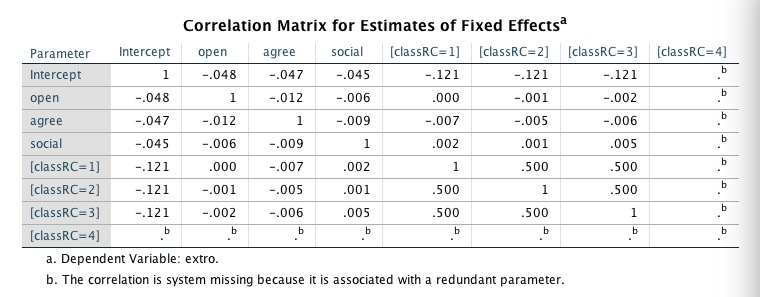
\includegraphics{correlation.jpeg}\\

\end{frame}

\begin{frame}{Conclusion}

\begin{itemize}
\item
  Linear mixed effect model is an useful model for real-world analysis
\item
\item
\end{itemize}

\end{frame}

\begin{frame}{Reference}

\begin{itemize}
\item
  \url{http://bayes.acs.unt.edu:8083/BayesContent/class/Jon/SPSS_SC/Module9/M9_LMM/SPSS_M9_LMM.htm}
\item
  \url{http://users.stat.umn.edu/~helwig/notes/lmer-Notes.pdf}
\item
  \url{http://www.bodowinter.com/tutorial/bw_LME_tutorial2.pdf}
\end{itemize}

\end{frame}

\end{document}
